% Options for packages loaded elsewhere
\PassOptionsToPackage{unicode}{hyperref}
\PassOptionsToPackage{hyphens}{url}
\PassOptionsToPackage{dvipsnames,svgnames,x11names}{xcolor}
%
\documentclass[
  letterpaper,
  DIV=11,
  numbers=noendperiod]{scrartcl}

\usepackage{amsmath,amssymb}
\usepackage{iftex}
\ifPDFTeX
  \usepackage[T1]{fontenc}
  \usepackage[utf8]{inputenc}
  \usepackage{textcomp} % provide euro and other symbols
\else % if luatex or xetex
  \usepackage{unicode-math}
  \defaultfontfeatures{Scale=MatchLowercase}
  \defaultfontfeatures[\rmfamily]{Ligatures=TeX,Scale=1}
\fi
\usepackage{lmodern}
\ifPDFTeX\else  
    % xetex/luatex font selection
\fi
% Use upquote if available, for straight quotes in verbatim environments
\IfFileExists{upquote.sty}{\usepackage{upquote}}{}
\IfFileExists{microtype.sty}{% use microtype if available
  \usepackage[]{microtype}
  \UseMicrotypeSet[protrusion]{basicmath} % disable protrusion for tt fonts
}{}
\makeatletter
\@ifundefined{KOMAClassName}{% if non-KOMA class
  \IfFileExists{parskip.sty}{%
    \usepackage{parskip}
  }{% else
    \setlength{\parindent}{0pt}
    \setlength{\parskip}{6pt plus 2pt minus 1pt}}
}{% if KOMA class
  \KOMAoptions{parskip=half}}
\makeatother
\usepackage{xcolor}
\setlength{\emergencystretch}{3em} % prevent overfull lines
\setcounter{secnumdepth}{-\maxdimen} % remove section numbering
% Make \paragraph and \subparagraph free-standing
\ifx\paragraph\undefined\else
  \let\oldparagraph\paragraph
  \renewcommand{\paragraph}[1]{\oldparagraph{#1}\mbox{}}
\fi
\ifx\subparagraph\undefined\else
  \let\oldsubparagraph\subparagraph
  \renewcommand{\subparagraph}[1]{\oldsubparagraph{#1}\mbox{}}
\fi

\usepackage{color}
\usepackage{fancyvrb}
\newcommand{\VerbBar}{|}
\newcommand{\VERB}{\Verb[commandchars=\\\{\}]}
\DefineVerbatimEnvironment{Highlighting}{Verbatim}{commandchars=\\\{\}}
% Add ',fontsize=\small' for more characters per line
\usepackage{framed}
\definecolor{shadecolor}{RGB}{241,243,245}
\newenvironment{Shaded}{\begin{snugshade}}{\end{snugshade}}
\newcommand{\AlertTok}[1]{\textcolor[rgb]{0.68,0.00,0.00}{#1}}
\newcommand{\AnnotationTok}[1]{\textcolor[rgb]{0.37,0.37,0.37}{#1}}
\newcommand{\AttributeTok}[1]{\textcolor[rgb]{0.40,0.45,0.13}{#1}}
\newcommand{\BaseNTok}[1]{\textcolor[rgb]{0.68,0.00,0.00}{#1}}
\newcommand{\BuiltInTok}[1]{\textcolor[rgb]{0.00,0.23,0.31}{#1}}
\newcommand{\CharTok}[1]{\textcolor[rgb]{0.13,0.47,0.30}{#1}}
\newcommand{\CommentTok}[1]{\textcolor[rgb]{0.37,0.37,0.37}{#1}}
\newcommand{\CommentVarTok}[1]{\textcolor[rgb]{0.37,0.37,0.37}{\textit{#1}}}
\newcommand{\ConstantTok}[1]{\textcolor[rgb]{0.56,0.35,0.01}{#1}}
\newcommand{\ControlFlowTok}[1]{\textcolor[rgb]{0.00,0.23,0.31}{#1}}
\newcommand{\DataTypeTok}[1]{\textcolor[rgb]{0.68,0.00,0.00}{#1}}
\newcommand{\DecValTok}[1]{\textcolor[rgb]{0.68,0.00,0.00}{#1}}
\newcommand{\DocumentationTok}[1]{\textcolor[rgb]{0.37,0.37,0.37}{\textit{#1}}}
\newcommand{\ErrorTok}[1]{\textcolor[rgb]{0.68,0.00,0.00}{#1}}
\newcommand{\ExtensionTok}[1]{\textcolor[rgb]{0.00,0.23,0.31}{#1}}
\newcommand{\FloatTok}[1]{\textcolor[rgb]{0.68,0.00,0.00}{#1}}
\newcommand{\FunctionTok}[1]{\textcolor[rgb]{0.28,0.35,0.67}{#1}}
\newcommand{\ImportTok}[1]{\textcolor[rgb]{0.00,0.46,0.62}{#1}}
\newcommand{\InformationTok}[1]{\textcolor[rgb]{0.37,0.37,0.37}{#1}}
\newcommand{\KeywordTok}[1]{\textcolor[rgb]{0.00,0.23,0.31}{#1}}
\newcommand{\NormalTok}[1]{\textcolor[rgb]{0.00,0.23,0.31}{#1}}
\newcommand{\OperatorTok}[1]{\textcolor[rgb]{0.37,0.37,0.37}{#1}}
\newcommand{\OtherTok}[1]{\textcolor[rgb]{0.00,0.23,0.31}{#1}}
\newcommand{\PreprocessorTok}[1]{\textcolor[rgb]{0.68,0.00,0.00}{#1}}
\newcommand{\RegionMarkerTok}[1]{\textcolor[rgb]{0.00,0.23,0.31}{#1}}
\newcommand{\SpecialCharTok}[1]{\textcolor[rgb]{0.37,0.37,0.37}{#1}}
\newcommand{\SpecialStringTok}[1]{\textcolor[rgb]{0.13,0.47,0.30}{#1}}
\newcommand{\StringTok}[1]{\textcolor[rgb]{0.13,0.47,0.30}{#1}}
\newcommand{\VariableTok}[1]{\textcolor[rgb]{0.07,0.07,0.07}{#1}}
\newcommand{\VerbatimStringTok}[1]{\textcolor[rgb]{0.13,0.47,0.30}{#1}}
\newcommand{\WarningTok}[1]{\textcolor[rgb]{0.37,0.37,0.37}{\textit{#1}}}

\providecommand{\tightlist}{%
  \setlength{\itemsep}{0pt}\setlength{\parskip}{0pt}}\usepackage{longtable,booktabs,array}
\usepackage{calc} % for calculating minipage widths
% Correct order of tables after \paragraph or \subparagraph
\usepackage{etoolbox}
\makeatletter
\patchcmd\longtable{\par}{\if@noskipsec\mbox{}\fi\par}{}{}
\makeatother
% Allow footnotes in longtable head/foot
\IfFileExists{footnotehyper.sty}{\usepackage{footnotehyper}}{\usepackage{footnote}}
\makesavenoteenv{longtable}
\usepackage{graphicx}
\makeatletter
\def\maxwidth{\ifdim\Gin@nat@width>\linewidth\linewidth\else\Gin@nat@width\fi}
\def\maxheight{\ifdim\Gin@nat@height>\textheight\textheight\else\Gin@nat@height\fi}
\makeatother
% Scale images if necessary, so that they will not overflow the page
% margins by default, and it is still possible to overwrite the defaults
% using explicit options in \includegraphics[width, height, ...]{}
\setkeys{Gin}{width=\maxwidth,height=\maxheight,keepaspectratio}
% Set default figure placement to htbp
\makeatletter
\def\fps@figure{htbp}
\makeatother

\usepackage{fontspec}
\usepackage{multirow}
\usepackage{multicol}
\usepackage{colortbl}
\usepackage{hhline}
\newlength\Oldarrayrulewidth
\newlength\Oldtabcolsep
\usepackage{longtable}
\usepackage{array}
\usepackage{hyperref}
\usepackage{float}
\usepackage{wrapfig}
\KOMAoption{captions}{tableheading}
\makeatletter
\makeatother
\makeatletter
\makeatother
\makeatletter
\@ifpackageloaded{caption}{}{\usepackage{caption}}
\AtBeginDocument{%
\ifdefined\contentsname
  \renewcommand*\contentsname{Table of contents}
\else
  \newcommand\contentsname{Table of contents}
\fi
\ifdefined\listfigurename
  \renewcommand*\listfigurename{List of Figures}
\else
  \newcommand\listfigurename{List of Figures}
\fi
\ifdefined\listtablename
  \renewcommand*\listtablename{List of Tables}
\else
  \newcommand\listtablename{List of Tables}
\fi
\ifdefined\figurename
  \renewcommand*\figurename{Figure}
\else
  \newcommand\figurename{Figure}
\fi
\ifdefined\tablename
  \renewcommand*\tablename{Table}
\else
  \newcommand\tablename{Table}
\fi
}
\@ifpackageloaded{float}{}{\usepackage{float}}
\floatstyle{ruled}
\@ifundefined{c@chapter}{\newfloat{codelisting}{h}{lop}}{\newfloat{codelisting}{h}{lop}[chapter]}
\floatname{codelisting}{Listing}
\newcommand*\listoflistings{\listof{codelisting}{List of Listings}}
\makeatother
\makeatletter
\@ifpackageloaded{caption}{}{\usepackage{caption}}
\@ifpackageloaded{subcaption}{}{\usepackage{subcaption}}
\makeatother
\makeatletter
\@ifpackageloaded{tcolorbox}{}{\usepackage[skins,breakable]{tcolorbox}}
\makeatother
\makeatletter
\@ifundefined{shadecolor}{\definecolor{shadecolor}{rgb}{.97, .97, .97}}
\makeatother
\makeatletter
\makeatother
\makeatletter
\makeatother
\ifLuaTeX
  \usepackage{selnolig}  % disable illegal ligatures
\fi
\IfFileExists{bookmark.sty}{\usepackage{bookmark}}{\usepackage{hyperref}}
\IfFileExists{xurl.sty}{\usepackage{xurl}}{} % add URL line breaks if available
\urlstyle{same} % disable monospaced font for URLs
\hypersetup{
  pdftitle={Homework 4},
  pdfauthor={Kyle Cahitas},
  colorlinks=true,
  linkcolor={blue},
  filecolor={Maroon},
  citecolor={Blue},
  urlcolor={Blue},
  pdfcreator={LaTeX via pandoc}}

\title{Homework 4}
\author{Kyle Cahitas}
\date{2023-05-25}

\begin{document}
\maketitle
\ifdefined\Shaded\renewenvironment{Shaded}{\begin{tcolorbox}[enhanced, breakable, boxrule=0pt, sharp corners, frame hidden, interior hidden, borderline west={3pt}{0pt}{shadecolor}]}{\end{tcolorbox}}\fi

\hypertarget{question--how-does-fish-length-predict-fish-weight-for-trout-perch-across-all-sample-years}{%
\subsection{Question- How does fish length predict fish weight for trout
perch (across all sample
years)}\label{question--how-does-fish-length-predict-fish-weight-for-trout-perch-across-all-sample-years}}

\begin{Shaded}
\begin{Highlighting}[]
\CommentTok{\#filtering data, importing csv}
\NormalTok{fish\_df }\OtherTok{\textless{}{-}} \FunctionTok{read\_csv}\NormalTok{(}\FunctionTok{here}\NormalTok{(}\StringTok{"data"}\NormalTok{, }\StringTok{"ntl6\_v12.csv"}\NormalTok{)) }\SpecialCharTok{\%\textgreater{}\%} 
  
  \CommentTok{\#filtering rows that have "TROUTPERCH}
  \FunctionTok{filter}\NormalTok{(spname }\SpecialCharTok{==} \StringTok{"TROUTPERCH"}\NormalTok{) }\SpecialCharTok{\%\textgreater{}\%} 
  
  \CommentTok{\#selecting specific rows}
  \FunctionTok{select}\NormalTok{(spname,year4,length,weight) }\SpecialCharTok{\%\textgreater{}\%} 
  
  \CommentTok{\#renaming columnns }
  \FunctionTok{rename}\NormalTok{(}\AttributeTok{year =}\NormalTok{ year4)}
\end{Highlighting}
\end{Shaded}

\begin{verbatim}
Rows: 349229 Columns: 15
-- Column specification --------------------------------------------------------
Delimiter: ","
chr  (8): lakeid, gearid, spname, sampletype, indid, fishpart, spseq, flag
dbl  (5): year4, depth, rep, length, weight
lgl  (1): sex
date (1): sampledate

i Use `spec()` to retrieve the full column specification for this data.
i Specify the column types or set `show_col_types = FALSE` to quiet this message.
\end{verbatim}

1.Hypothesis

Linear models describes linear relationship between variable and
predictor

Null Hypothesis: There is no significant relationship between
trout-perch length (mm) and trout-perch weight (g), indicating that
trout-perch length does not indicate trout-perch weight. There is no
significant relationship between trout-perch length (mm) and trout perch
weight (g), due to the slope of the regression line result to zero or
the p-value was greater than 0.05.

Alternative Hypothesis: There is significant relationship between
trout-perch length (mm) and trout-perch weight (g), indicating that
trout-perch length can predict trout-perch weight. There is significant
relationship between trout-perch length (mm) and trout-perch weight (g),
due to the slope of the regression line resulting to not equal zero and
having a p-value lower than 0.05.

\begin{enumerate}
\def\labelenumi{\arabic{enumi}.}
\setcounter{enumi}{1}
\tightlist
\item
\end{enumerate}

\begin{Shaded}
\begin{Highlighting}[]
\CommentTok{\# 200 missing rows for weight}
\CommentTok{\# have all rows for length }
\FunctionTok{gg\_miss\_var}\NormalTok{(fish\_df) }
\end{Highlighting}
\end{Shaded}

\begin{figure}[H]

{\centering 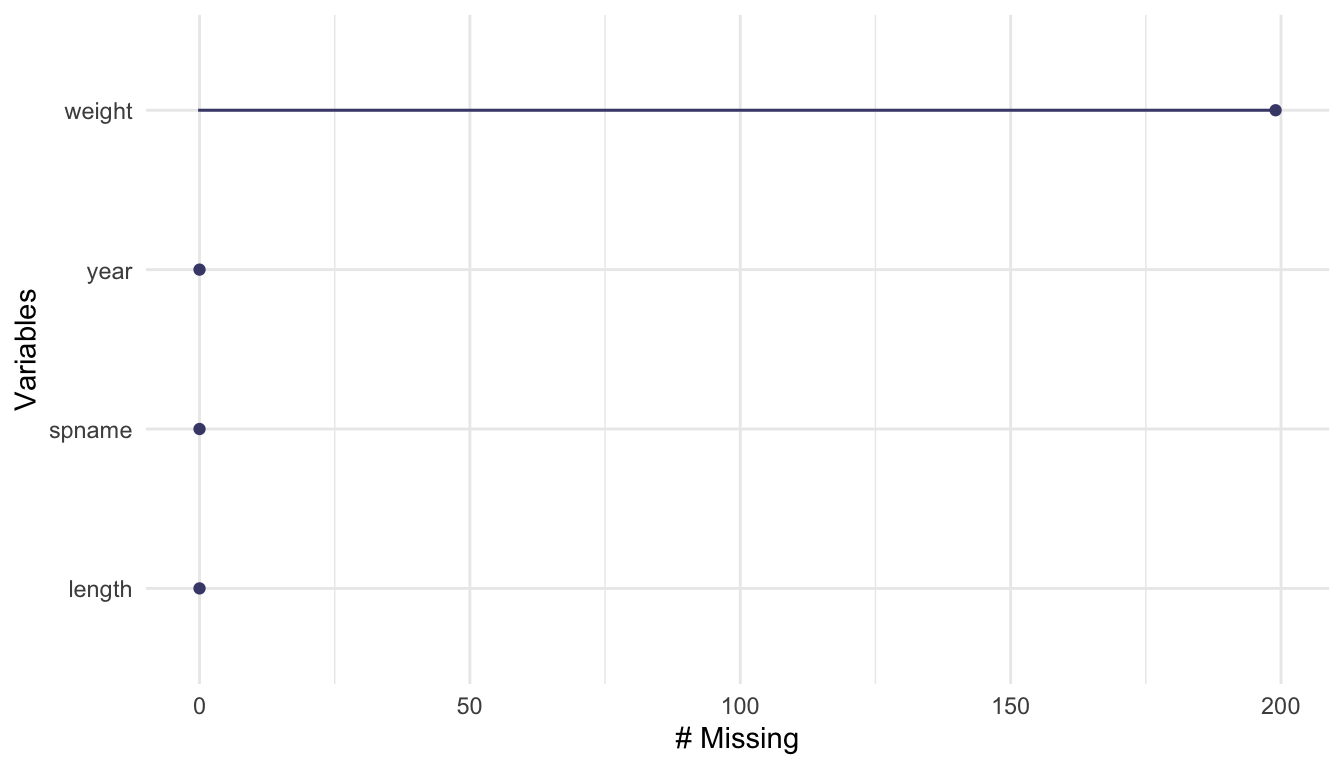
\includegraphics[width=0.9\textwidth,height=\textheight]{homework-4_files/figure-pdf/missing-data-vis-1.pdf}

}

\end{figure}

When running the function gg\_miss\_var, a total of 199 missing
observation was discovered in the column of weight. This resulted in
having the original data frame be 489 to the new data frame being 290.
These missing observation help assign weight be the depending variable
and length being the independent variable.

\begin{enumerate}
\def\labelenumi{\arabic{enumi}.}
\setcounter{enumi}{2}
\tightlist
\item
\end{enumerate}

\begin{Shaded}
\begin{Highlighting}[]
\CommentTok{\#using tidyverse to filter out any Na values in the weight column \# and deleting that row in the process}
\NormalTok{troutperch\_Na }\OtherTok{\textless{}{-}}\NormalTok{ fish\_df }\SpecialCharTok{\%\textgreater{}\%} 
  \FunctionTok{drop\_na}\NormalTok{(weight)}

\CommentTok{\#View(troutperch\_Na)}
\end{Highlighting}
\end{Shaded}

\begin{Shaded}
\begin{Highlighting}[]
\CommentTok{\#quick visual of the data }
\FunctionTok{ggplot}\NormalTok{(}\AttributeTok{data =}\NormalTok{ troutperch\_Na, }\FunctionTok{aes}\NormalTok{(}\AttributeTok{x =}\NormalTok{ length, }\AttributeTok{y =}\NormalTok{ weight)) }\SpecialCharTok{+} 
  
  \FunctionTok{geom\_point}\NormalTok{()}\SpecialCharTok{+}
  
  \FunctionTok{labs}\NormalTok{(}\AttributeTok{title =} \StringTok{"Trout{-}perch lengths and weight"}\NormalTok{)}\SpecialCharTok{+}
  
  \FunctionTok{theme\_classic}\NormalTok{()}
\end{Highlighting}
\end{Shaded}

\begin{figure}[H]

{\centering 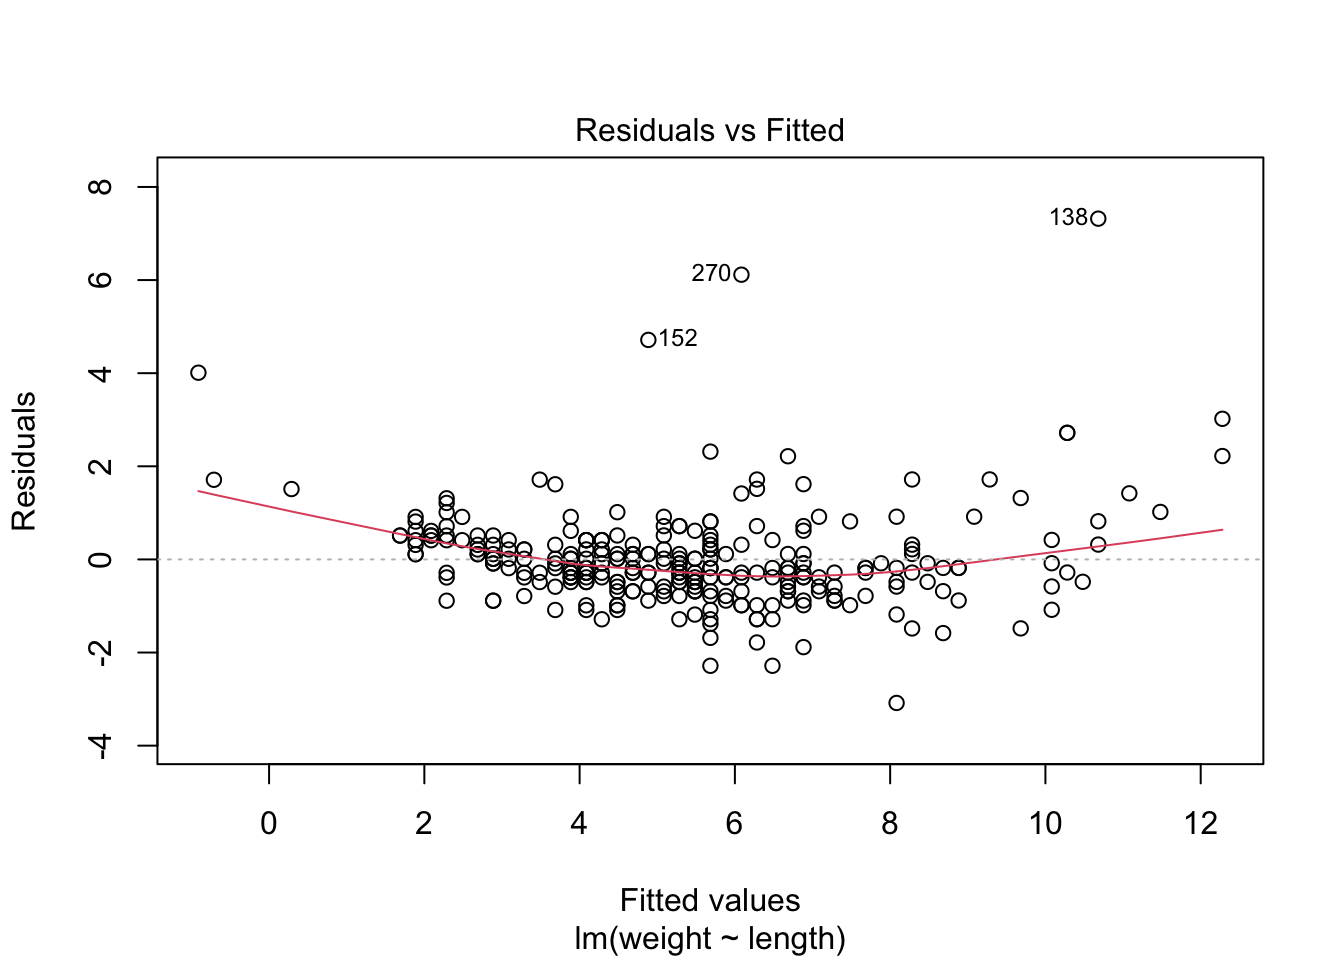
\includegraphics[width=0.9\textwidth,height=\textheight]{homework-4_files/figure-pdf/unnamed-chunk-2-1.pdf}

}

\end{figure}

By looking at a quick visual of the data, there appears to be a somewhat
postive slope, but more tests need to be done.

\begin{enumerate}
\def\labelenumi{\arabic{enumi}.}
\setcounter{enumi}{4}
\tightlist
\item
  Diagnostic Plot
\end{enumerate}

\begin{Shaded}
\begin{Highlighting}[]
\CommentTok{\#diagnostic plot}
\NormalTok{modelobject }\OtherTok{\textless{}{-}} \FunctionTok{lm}\NormalTok{(weight }\SpecialCharTok{\textasciitilde{}}\NormalTok{ length, }\AttributeTok{data =}\NormalTok{ troutperch\_Na)}

\CommentTok{\#combining all four groups in a 2 x 2}
\FunctionTok{par}\NormalTok{(}\AttributeTok{mfrow =} \FunctionTok{c}\NormalTok{(}\DecValTok{2}\NormalTok{,}\DecValTok{2}\NormalTok{))}

\FunctionTok{plot}\NormalTok{(modelobject)}
\end{Highlighting}
\end{Shaded}

\begin{figure}[H]

{\centering \includegraphics{homework-4_files/figure-pdf/diagnostic-plot-1.pdf}

}

\end{figure}

The diagnostic plot ``Residual vs Fitted'' visually implies that the
data is heteroscedasticity. The observations are clumped in the middle
and are not scattered.

The diagnostic plot ``Normal Q-Q'' visually implies that data is normal
but the right tail is very close to not being normal.

The diagnostic plot ``Scale-Location visually implies if the data is
heteroscedasiticty or homoscedasticity. Again, majority of the data
resides in the middle, concluding that the data is of
heteroscedasiticity.

The diagnostic plot ``Residual vs Leverage'' visually implies if there
any outlier within the data. There appears to be one data point that is
outside of the dashed line and thus, a outlier.

\begin{enumerate}
\def\labelenumi{\arabic{enumi}.}
\setcounter{enumi}{5}
\tightlist
\item
  Summary
\end{enumerate}

\begin{Shaded}
\begin{Highlighting}[]
\CommentTok{\#using function summary() to display results }
\NormalTok{model\_summary }\OtherTok{\textless{}{-}} \FunctionTok{summary}\NormalTok{(modelobject)}

\NormalTok{model\_summary}
\end{Highlighting}
\end{Shaded}

\begin{verbatim}

Call:
lm(formula = weight ~ length, data = troutperch_Na)

Residuals:
    Min      1Q  Median      3Q     Max 
-3.0828 -0.4862 -0.1830  0.4128  7.3191 

Coefficients:
              Estimate Std. Error t value Pr(>|t|)    
(Intercept) -11.702476   0.481564  -24.30   <2e-16 ***
length        0.199852   0.005584   35.79   <2e-16 ***
---
Signif. codes:  0 '***' 0.001 '**' 0.01 '*' 0.05 '.' 0.1 ' ' 1

Residual standard error: 1.057 on 288 degrees of freedom
Multiple R-squared:  0.8164,    Adjusted R-squared:  0.8158 
F-statistic:  1281 on 1 and 288 DF,  p-value: < 2.2e-16
\end{verbatim}

The function summary

\begin{enumerate}
\def\labelenumi{\arabic{enumi}.}
\setcounter{enumi}{6}
\tightlist
\item
  ANOVA
\end{enumerate}

\begin{Shaded}
\begin{Highlighting}[]
\CommentTok{\#anova is used to get analysis of variance tables for a model }
\NormalTok{model\_sqaures }\OtherTok{\textless{}{-}} \FunctionTok{anova}\NormalTok{(modelobject)}
\end{Highlighting}
\end{Shaded}

\begin{Shaded}
\begin{Highlighting}[]
\CommentTok{\#creating a table that demonstrates ANOVA}
\NormalTok{model\_squares\_table }\OtherTok{\textless{}{-}}\FunctionTok{tidy}\NormalTok{(model\_sqaures) }\SpecialCharTok{\%\textgreater{}\%} 
  \CommentTok{\# round the sum of squares and mean squares columns to have 5 digits (could be less)}
  \FunctionTok{mutate}\NormalTok{(}\FunctionTok{across}\NormalTok{(sumsq}\SpecialCharTok{:}\NormalTok{meansq, }\SpecialCharTok{\textasciitilde{}} \FunctionTok{round}\NormalTok{(.x, }\AttributeTok{digits =} \DecValTok{5}\NormalTok{))) }\SpecialCharTok{\%\textgreater{}\%} 
  \CommentTok{\# round the F{-}statistic to have 1 digit}
  \FunctionTok{mutate}\NormalTok{(}\AttributeTok{statistic =} \FunctionTok{round}\NormalTok{(statistic, }\AttributeTok{digits =} \DecValTok{1}\NormalTok{)) }\SpecialCharTok{\%\textgreater{}\%} 
  \CommentTok{\# replace the very very very small p value with \textless{} 0.001}
  
  \FunctionTok{mutate}\NormalTok{(}\AttributeTok{p.value =} \FunctionTok{case\_when}\NormalTok{(p.value }\SpecialCharTok{\textless{}}\FloatTok{0.001} \SpecialCharTok{\textasciitilde{}} \StringTok{"\textless{}0.001"}\NormalTok{)) }\SpecialCharTok{\%\textgreater{}\%} 
  
  \CommentTok{\#creating a table }
  \FunctionTok{flextable}\NormalTok{() }\SpecialCharTok{\%\textgreater{}\%} 
  
  \CommentTok{\#changing the header, for ease of understanding }
  \FunctionTok{set\_header\_labels}\NormalTok{(}\AttributeTok{df =} \StringTok{"Degrees of Freedom"}\NormalTok{, }
                    \AttributeTok{sumsq =} \StringTok{"Sum of squares"}\NormalTok{,}
                    \AttributeTok{meansq =} \StringTok{"Mean squares"}\NormalTok{,}
                    \AttributeTok{statistic =} \StringTok{"F{-}statistic"}\NormalTok{,}
                    \AttributeTok{p.value =} \StringTok{"p{-}value"}
\NormalTok{                    )}
\NormalTok{model\_squares\_table}
\end{Highlighting}
\end{Shaded}

\global\setlength{\Oldarrayrulewidth}{\arrayrulewidth}

\global\setlength{\Oldtabcolsep}{\tabcolsep}

\setlength{\tabcolsep}{0pt}

\renewcommand*{\arraystretch}{1.5}



\providecommand{\ascline}[3]{\noalign{\global\arrayrulewidth #1}\arrayrulecolor[HTML]{#2}\cline{#3}}

\begin{longtable*}[c]{|p{0.75in}|p{0.75in}|p{0.75in}|p{0.75in}|p{0.75in}|p{0.75in}}



\ascline{1.5pt}{666666}{1-6}

\multicolumn{1}{>{\raggedright}m{\dimexpr 0.75in+0\tabcolsep}}{\textcolor[HTML]{000000}{\fontsize{11}{11}\selectfont{term}}} & \multicolumn{1}{>{\raggedleft}m{\dimexpr 0.75in+0\tabcolsep}}{\textcolor[HTML]{000000}{\fontsize{11}{11}\selectfont{Degrees\ of\ Freedom}}} & \multicolumn{1}{>{\raggedleft}m{\dimexpr 0.75in+0\tabcolsep}}{\textcolor[HTML]{000000}{\fontsize{11}{11}\selectfont{Sum\ of\ squares}}} & \multicolumn{1}{>{\raggedleft}m{\dimexpr 0.75in+0\tabcolsep}}{\textcolor[HTML]{000000}{\fontsize{11}{11}\selectfont{Mean\ squares}}} & \multicolumn{1}{>{\raggedleft}m{\dimexpr 0.75in+0\tabcolsep}}{\textcolor[HTML]{000000}{\fontsize{11}{11}\selectfont{F-statistic}}} & \multicolumn{1}{>{\raggedright}m{\dimexpr 0.75in+0\tabcolsep}}{\textcolor[HTML]{000000}{\fontsize{11}{11}\selectfont{p-value}}} \\

\ascline{1.5pt}{666666}{1-6}\endhead



\multicolumn{1}{>{\raggedright}m{\dimexpr 0.75in+0\tabcolsep}}{\textcolor[HTML]{000000}{\fontsize{11}{11}\selectfont{length}}} & \multicolumn{1}{>{\raggedleft}m{\dimexpr 0.75in+0\tabcolsep}}{\textcolor[HTML]{000000}{\fontsize{11}{11}\selectfont{1}}} & \multicolumn{1}{>{\raggedleft}m{\dimexpr 0.75in+0\tabcolsep}}{\textcolor[HTML]{000000}{\fontsize{11}{11}\selectfont{1,432.2877}}} & \multicolumn{1}{>{\raggedleft}m{\dimexpr 0.75in+0\tabcolsep}}{\textcolor[HTML]{000000}{\fontsize{11}{11}\selectfont{1,432.28769}}} & \multicolumn{1}{>{\raggedleft}m{\dimexpr 0.75in+0\tabcolsep}}{\textcolor[HTML]{000000}{\fontsize{11}{11}\selectfont{1,280.8}}} & \multicolumn{1}{>{\raggedright}m{\dimexpr 0.75in+0\tabcolsep}}{\textcolor[HTML]{000000}{\fontsize{11}{11}\selectfont{<0.001}}} \\





\multicolumn{1}{>{\raggedright}m{\dimexpr 0.75in+0\tabcolsep}}{\textcolor[HTML]{000000}{\fontsize{11}{11}\selectfont{Residuals}}} & \multicolumn{1}{>{\raggedleft}m{\dimexpr 0.75in+0\tabcolsep}}{\textcolor[HTML]{000000}{\fontsize{11}{11}\selectfont{288}}} & \multicolumn{1}{>{\raggedleft}m{\dimexpr 0.75in+0\tabcolsep}}{\textcolor[HTML]{000000}{\fontsize{11}{11}\selectfont{322.0525}}} & \multicolumn{1}{>{\raggedleft}m{\dimexpr 0.75in+0\tabcolsep}}{\textcolor[HTML]{000000}{\fontsize{11}{11}\selectfont{1.11824}}} & \multicolumn{1}{>{\raggedleft}m{\dimexpr 0.75in+0\tabcolsep}}{\textcolor[HTML]{000000}{\fontsize{11}{11}\selectfont{}}} & \multicolumn{1}{>{\raggedright}m{\dimexpr 0.75in+0\tabcolsep}}{\textcolor[HTML]{000000}{\fontsize{11}{11}\selectfont{}}} \\

\ascline{1.5pt}{666666}{1-6}



\end{longtable*}



\arrayrulecolor[HTML]{000000}

\global\setlength{\arrayrulewidth}{\Oldarrayrulewidth}

\global\setlength{\tabcolsep}{\Oldtabcolsep}

\renewcommand*{\arraystretch}{1}

8.In 1-2 sentences, describe how the ANOVA table relates to the
information you get from the summary() object.

The ANOVA tables relates to the summary() object, in terms of finding if
the slope is equal to zero or not equal to zero. By incorporating sum of
squares and mean squares, the F-value if the value is large means that
the variation among group means is more than expected by chance, and can
conclude that the slope is not equal to zero.

9.In 2-3 sentences, summarize your results in prose with in-text
references to test results. Include all relevant information.

When running the summary(), the t-value for length was 35.79, the
length's slope was 0.19985, p-value was \textless2e-16 and the standard
error was 0.005585. When running the ANOVA the F-test was 1,280.8 and
p-value was less than 0.001. The results from both tests, concluded that
the length slope is postive, has a p-value lower than 0.05, thus we can
reject the null hypothesis and accept the alternative hypothesis and can
conclude that fish length can predict fish weight for trout perch.

\begin{enumerate}
\def\labelenumi{\arabic{enumi}.}
\setcounter{enumi}{9}
\tightlist
\item
  Model Prediction Plot
\end{enumerate}

\begin{Shaded}
\begin{Highlighting}[]
\NormalTok{predictions }\OtherTok{\textless{}{-}} \FunctionTok{ggpredict}\NormalTok{(modelobject, }\AttributeTok{terms =} \StringTok{"length"}\NormalTok{)}

\FunctionTok{View}\NormalTok{(predictions)}
\end{Highlighting}
\end{Shaded}

\begin{Shaded}
\begin{Highlighting}[]
\NormalTok{plot\_predictions }\OtherTok{\textless{}{-}} \FunctionTok{ggplot}\NormalTok{(}\AttributeTok{data =}\NormalTok{ troutperch\_Na, }
                           \FunctionTok{aes}\NormalTok{(}\AttributeTok{x =}\NormalTok{ length, }\AttributeTok{y =}\NormalTok{ weight)) }\SpecialCharTok{+}
  \CommentTok{\#type of graph   }
  \FunctionTok{geom\_point}\NormalTok{() }\SpecialCharTok{+}
  \CommentTok{\# plotting the predictions on data }
  \FunctionTok{geom\_line}\NormalTok{(}\AttributeTok{data =}\NormalTok{ predictions, }
            \FunctionTok{aes}\NormalTok{(}\AttributeTok{x =}\NormalTok{ x, }\AttributeTok{y =}\NormalTok{ predicted), }
            \AttributeTok{color =} \StringTok{"brown"}\NormalTok{, }\AttributeTok{linewidth =}\NormalTok{ .}\DecValTok{9}\NormalTok{) }\SpecialCharTok{+}
  
  \CommentTok{\# then plot the 95\% confidence interval from ggpredict}
  \FunctionTok{geom\_ribbon}\NormalTok{(}\AttributeTok{data =}\NormalTok{ predictions, }
              \FunctionTok{aes}\NormalTok{(}\AttributeTok{x =}\NormalTok{ x, }\AttributeTok{y =}\NormalTok{ predicted, }\AttributeTok{ymin =}\NormalTok{ conf.low, }\AttributeTok{ymax =}\NormalTok{ conf.high), }
              \AttributeTok{alpha =}\NormalTok{ .}\DecValTok{2}\NormalTok{) }\SpecialCharTok{+}
  
  \DocumentationTok{\#\# theme and labels \#\#}
 \FunctionTok{theme\_economist}\NormalTok{()}\SpecialCharTok{+} \CommentTok{\#from ggthemes }
  
 \CommentTok{\# labeling plot }
 \FunctionTok{labs}\NormalTok{(}\AttributeTok{x =} \StringTok{"Length (mm)"}\NormalTok{,}
      \AttributeTok{y =} \StringTok{"Weight (g)"}\NormalTok{,}
      \AttributeTok{title =} \StringTok{"Prediction of Trout{-}Perch"}
\NormalTok{      )}\SpecialCharTok{+} 
  \CommentTok{\#adjusting functions }
  \FunctionTok{theme}\NormalTok{(}
    \AttributeTok{plot.title =} \FunctionTok{element\_text}\NormalTok{(}\AttributeTok{face =} \StringTok{"bold"}\NormalTok{),}
    \AttributeTok{axis.ticks =} \FunctionTok{element\_line}\NormalTok{(}\AttributeTok{linewidth =} \DecValTok{3}\NormalTok{, }\AttributeTok{color =} \StringTok{"darkgray"}\NormalTok{)}
\NormalTok{  )}
 
\NormalTok{plot\_predictions}
\end{Highlighting}
\end{Shaded}

\begin{figure}[H]

{\centering 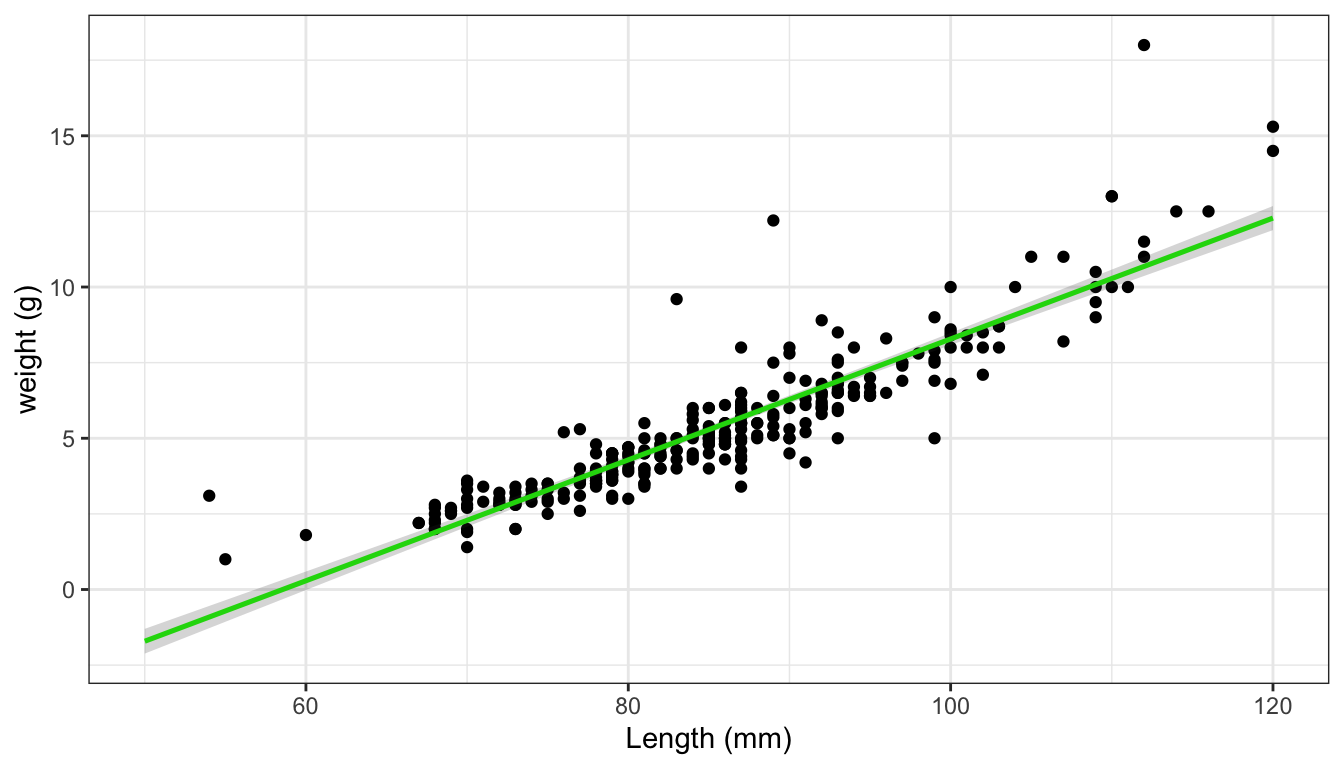
\includegraphics[width=0.9\textwidth,height=\textheight]{homework-4_files/figure-pdf/unnamed-chunk-5-1.pdf}

}

\end{figure}

The plot above demonstrates data of trout perch weight and length,
between the years of 1981 - 2022 in the North Temperate Lakes. When
comparing the trout perch length and weight and by running ANOVA and the
summery(), the length has a postive slope. The predication interval is
visualized by the brown line which defines a range of values within
which a response is likely to fall given a specified length value. The
gray hue, surrounding the predication interval represents the a
confidence level of 95\% the predication interval can predict in. In
conclusion, the data can help predict the weight of a troutperch when
given the length of the troutperch.

The above plot demonstrates data regarding the weight and length of
trout perch in the North Temperate Lakes from 1981 to 2022. By conducing
ANOVA and using the ``summary()'' function, we had significant evidence
to reject the null hypothesis and accept the alternative hypothesis.
This is viewed being that the slope of this plot does not equal to zero
but the length of the trout perch exhibits a positive slop.

The brown line in the plot represents the prediction interval, which
establishes a range of values where the response is likely to fall,
given a specific length value. The gray shading surrounding the
prediction interval signifies a confidence level of 95\%, indicating the
accuracy of the prediction interval. In conclusion, this data can be
utilized to predict the weight of a trout perch based on its length in
the North Temperate Lakes.



\end{document}
